\documentclass[../../main.tex]{subfiles}
\begin{document}

{\bf [解]}

% TODO: 四面体の様子
\begin{figure}[htb]
  \centering
  \begin{tikzpicture}[
      x={(-0.85cm, -0.45cm)}, % x軸: 左手前
      y={(1.25cm, 0.05cm)},   % y軸: 右
      z={(0cm, 1.45cm)},      % z軸: 真上
      scale=2.2, >=stealth, every node/.style={font=\small}
    ]

    % ============================================================
    % 1. 厳密な 3D 座標設定
    % p = sqrt(6) ≈ 2.4495, q = 1.0, r = sqrt(3) ≈ 1.7321
    % ============================================================
    \def\pVal{2.4495} % sqrt(6)
    \def\qVal{1.0}    % 1
    \def\rVal{1.7321} % sqrt(3)

    \coordinate (O) at (0, 0, 0);
    \coordinate (A) at (\pVal, 0, \rVal);
    \coordinate (B) at (\pVal, \qVal, 0);
    \coordinate (C) at (0, \qVal, \rVal);

    % 垂足 H = (5/9)*A - (1/3)*B (平面 L 上で三角形 OAB の外側)
    \coordinate (H) at ($ 5/9*(A) - 1/3*(B) $);

    % 直方体の補助頂点
    \coordinate (X1) at (\pVal, 0, 0);
    \coordinate (Y1) at (0, \qVal, 0);
    \coordinate (Z1) at (0, 0, \rVal);
    \coordinate (T)  at (\pVal, \qVal, \rVal);

    % ============================================================
    % 2. 平面 L (OAB を含む無限平面の有限表現シート)
    % H(5/9, -1/3) や O(0,0), A(1,0), B(0,1) を完全に内包する領域
    % α: -0.2 〜 1.15,  β: -0.55 〜 1.15
    % ============================================================
    \coordinate (PL_BL) at ($ -0.2*(A) - 0.55*(B) $);
    \coordinate (PL_BR) at ($ -0.2*(A) + 1.15*(B) $);
    \coordinate (PL_TR) at ($ 1.15*(A) + 1.15*(B) $);
    \coordinate (PL_TL) at ($ 1.15*(A) - 0.55*(B) $);

    % 平面 L 全体を薄い青で塗り広げる
    \fill[blue!8, opacity=0.6] (PL_BL) -- (PL_BR) -- (PL_TR) -- (PL_TL) -- cycle;
    \draw[thick, blue!50!black, dashed] (PL_BL) -- (PL_BR) -- (PL_TR) -- (PL_TL) -- cycle;
    \node[blue!80!black, font=\footnotesize\bfseries, above left] at (PL_TL) {平面 $L$ ($\alpha\vec{a}+\beta\vec{b}$)};

    % 四面体の底面 \triangle OAB の部分だけ少し濃くして区別
    \fill[blue!18, opacity=0.7] (O) -- (A) -- (B) -- cycle;

    % ============================================================
    % 3. 直方体の枠組み（スケッチ通りの破線）
    % ============================================================
    \draw[dashed, gray!80!black] (O) -- (Y1) -- (B) -- (X1) -- cycle;
    \draw[dashed, gray!80!black] (Z1) -- (C) -- (T) -- (A) -- cycle;
    \draw[dashed, gray!80!black] (O) -- (Z1);
    \draw[dashed, gray!80!black] (X1) -- (A);
    \draw[dashed, gray!80!black] (Y1) -- (C);
    \draw[dashed, gray!80!black] (B) -- (T);

    % ============================================================
    % 4. 座標軸 (x, y, z)
    % ============================================================
    \draw[dashed, gray!60] (0, -0.6, 0) -- (O); % y 軸の負方向（H側）
    \draw[->, thick, gray!80!black] (O) -- (\pVal + 0.5, 0, 0) node[below left] {$x$};
    \draw[->, thick, gray!80!black] (O) -- (0, \qVal + 0.6, 0) node[right] {$y$};
    \draw[->, thick, gray!80!black] (O) -- (0, 0, \rVal + 0.5) node[above] {$z$};
    \node[below left=1pt] at (O) {$O$};

    % 軸目盛り
    \fill[black] (\pVal, 0, 0) circle (1.0pt) node[below left=1pt, font=\scriptsize] {$\sqrt{6}$};
    \fill[black] (0, \qVal, 0) circle (1.0pt) node[below right=1pt, font=\scriptsize] {$1$};
    \fill[black] (0, 0, \rVal) circle (1.0pt) node[left=2pt, font=\scriptsize] {$\sqrt{3}$};

    % ============================================================
    % 5. 垂線 CH と 平面 L 上の線分 OH
    % ============================================================
    % 平面 L 上の線分 OH (H が平面上にあることを明示)
    \draw[line width=1.2pt, red!85!black, dashed] (O) -- (H);

    % 垂線 CH (C から H へ)
    \draw[line width=1.5pt, red!85!black] (C) -- (H)
    node[midway, right=3pt, font=\footnotesize\bfseries] {$CH \perp \text{平面 } L$};

    % 直角マーク (C - H - O)
    \coordinate (sqCH) at ($ (H)!0.18!(C) $);
    \coordinate (sqOH) at ($ (H)!0.18!(O) $);
    \draw[thin, gray!70!black]
    (sqCH) -- ($ (sqCH) + (sqOH) - (H) $) -- (sqOH);

    % ============================================================
    % 6. 四面体 OABC の稜線
    % ============================================================
    % 奥側の稜線 (破線)
    \draw[thick, dashed, gray!60] (O) -- (A);
    \draw[thick, dashed, gray!60] (O) -- (C);

    % 手前側の稜線 (太い実線)
    \draw[line width=1.4pt, gray!20!black] (O) -- (B);
    \draw[line width=1.4pt, gray!20!black] (O) -- (C);
    \draw[line width=1.4pt, gray!20!black] (A) -- (B);
    \draw[line width=1.4pt, gray!20!black] (A) -- (C);
    \draw[line width=1.4pt, gray!20!black] (B) -- (C);

    % ============================================================
    % 7. 頂点プロットとラベル
    % ============================================================
    \fill[black] (A) circle (1.3pt) node[left=2pt] {$A$};
    \fill[black] (B) circle (1.3pt) node[below right=1pt] {$B$};
    \fill[black] (C) circle (1.3pt) node[above right=1pt] {$C$};
    \fill[red!85!black] (H) circle (1.5pt)
    node[below left=2pt, red!90!black, font=\footnotesize\bfseries] {$H\left(\frac{5}{9}\vec{a}-\frac{1}{3}\vec{b}\right)$};

    % ============================================================
    % 8. 辺長の注釈（スケッチの数値）
    % ============================================================
    \node[font=\footnotesize] at ($(O)!0.5!(A) + (-0.2, 0, 0.1)$) {$3$};
    \node[font=\footnotesize] at ($(O)!0.5!(B) + (0.1, -0.2, 0)$) {$\sqrt{7}$};
    \node[font=\footnotesize] at ($(A)!0.5!(B) + (0.2, -0.1, 0)$) {$2$};
    \node[font=\footnotesize] at ($(B)!0.5!(C) + (0.2, 0, 0)$) {$2$};
    \node[font=\footnotesize] at ($(O)!0.5!(C) + (-0.1, 0.2, 0.1)$) {$\sqrt{7}$};

  \end{tikzpicture}
  \caption{直方体内部における四面体 $OABC$，拡張された平面 $L$，および外側にある垂足 $H$}
  \label{fig:tetrahedron_plane_L_extended}
\end{figure}

上図のように$O(0,0,0)$を原点とする空間座標をとる．
$p,q,r>0$に対して$A(p,0,r), B(p,q,0), C(0,q,r)$とおく．
\begin{align}
  |OA| = 3, |OB| = \sqrt{7}, |AB|= 2 \label{eq:1}
\end{align}
だから，
\begin{align}
  \begin{cases}
    p^2 + r^2 = 9 \\
    p^2 + q^2 = 7 \\
    q^2 + r^2 = 4
  \end{cases}
  \therefore
  p = \sqrt{6},
  q = 1,
  r = \sqrt{3} \label{eq:2}
\end{align}
である．点 X に対し，$\overrightarrow{OX} = \vec{x}$ とおくと\cref{eq:1,eq:2}より
\begin{align}
  \begin{cases}
    |\vec{a}| = 3, |\vec{b}|=\sqrt{7}, |\vec{c}|=2 \\
    \vec{a}\cdot\vec{c}=3, \vec{b}\cdot\vec{c}=1
  \end{cases} \label{eq:3}
\end{align}
である．

\paragraph{(1)}

% TODO: L(OAB), Hの図

$H$ は $L$ 上の点だから
\begin{align}
  \overrightarrow{OH} = \alpha \vec{a} + \beta \vec{b} \label{eq:4}
\end{align}
と表せる．$CH \perp L$ だから，$\overrightarrow{CH} \cdot \vec{a} = 0$ かつ $\overrightarrow{CH} \cdot \vec{b} = 0$ である．\cref{eq:4}を代入して
\begin{align}
  \begin{cases}
    (\alpha \vec{a} + \beta \vec{b} - \vec{c}) \cdot \vec{a} = 0 \\
    (\alpha \vec{a} + \beta \vec{b} - \vec{c}) \cdot \vec{b} = 0
  \end{cases}
\end{align}
となる．\cref{eq:3}を代入して
\begin{align}
  \begin{cases}
    9\alpha + 6\beta - 3 = 0 \\
    6\alpha + 7\beta - 1 = 0
  \end{cases} \therefore
  \begin{cases}
    \alpha = \dfrac{5}{9} \\
    \beta = -\dfrac{1}{3}
  \end{cases}
\end{align}
である．\cref{eq:4}より
\begin{align}
  \overrightarrow{OH} = \dfrac{5}{9}\vec{a} - \dfrac{1}{3}\vec{b} \label{eq:5}
\end{align}
である．

\paragraph{(2)}

% TODO: 図
\begin{figure}[htb]
  \centering
  \begin{tikzpicture}[scale=2.0, >=stealth, every node/.style={font=\small}]

    % ============================================================
    % 1. 四面体 OABC の基準座標（スケッチのアングル）
    % ============================================================
    \coordinate (O) at (0, 0);
    \coordinate (B) at (-1.6, 1.4);
    \coordinate (A) at (3.0, 1.5);
    \coordinate (C) at (2.4, 4.0);

    % 垂足 H = 5/9 A - 1/3 B (平面 OAB 上の点)
    \coordinate (H) at ($ 5/9*(A) - 1/3*(B) $);

    % ============================================================
    % 2. 比率パラメータ t, s の設定
    % s = (9/2) * t
    % スケッチで Rt が線分 OC 内に見えるよう t = 0.16 に設定 (s = 0.72)
    % ============================================================
    \def\tVal{0.16}
    \pgfmathsetmacro{\sVal}{4.5 * \tVal} % 0.72

    % Pt, Qt on OA, OB
    \coordinate (Pt) at ($ (O)! \tVal !(A) $);
    \coordinate (Qt) at ($ (O)! \tVal !(B) $);

    % Rt on OC (厳密に直線 OC 上)
    \coordinate (Rt) at ($ (O)! \sVal !(C) $);

    % Ht の定義:
    % (i) 直線 PtQt 上の点として Qt から Pt 方向に 1 + 1.5 = 2.5 倍伸ばす
    % これにより Q_t - P_t - H_t は厳密に同一直線上に並ぶ
    \coordinate (Ht) at ($ (Qt)! 2.5 !(Pt) $);

    % ============================================================
    % 3. 四面体 OABC の骨格線
    % ============================================================
    % 奥側の稜線 (破線)
    \draw[thick, dashed, gray!50] (B) -- (A);

    % 手前側の稜線 (実線)
    \draw[line width=1.2pt, gray!25!black] (O) -- (B);
    \draw[line width=1.2pt, gray!25!black] (O) -- (A);
    \draw[line width=1.2pt, gray!25!black] (O) -- (C);
    \draw[line width=1.2pt, gray!25!black] (B) -- (C);
    \draw[line width=1.2pt, gray!25!black] (A) -- (C);

    % ============================================================
    % 4. 直線 OH と 垂線 CH (O - Ht - H の共線性を明示)
    % ============================================================
    % 直線 OH (O から H まで真っ直ぐ引くことで Ht を通過)
    \draw[line width=1.1pt, teal!70!black, dashed] (O) -- (H);

    % 垂線 CH (C から H へ)
    \draw[line width=1.1pt, gray!60, dashed] (C) -- (H);

    % ============================================================
    % 5. 切断面 M (Rt, Ht, Pt, Qt が同一平面上にある様子)
    % ============================================================
    % 直線 PtQtHt (Qt から Ht を越えて少し先まで真っ直ぐ引く)
    \draw[line width=1.3pt, blue!85!black] (Qt) -- (Pt);
    \draw[line width=1.2pt, blue!85!black, dashed] (Pt) -- ($ (Pt)! 1.25 !(Ht) $)
    node[right, font=\scriptsize] {直線 $P_tQ_t$};

    % 切断面三角形 PtQtRt (半透明の塗りつぶし)
    \fill[red!15, opacity=0.4] (Pt) -- (Qt) -- (Rt) -- cycle;
    \draw[line width=1.3pt, red!85!black] (Rt) -- (Pt);
    \draw[line width=1.3pt, red!85!black] (Rt) -- (Qt);

    % 垂線 RtHt (Rt から直線 PtQt 上の足 Ht へ下りる)
    \draw[line width=1.5pt, teal!85!black] (Rt) -- (Ht);

    % 直角マーク (Rt - Ht - 直線 PtQt)
    \coordinate (sqTop)  at ($ (Ht)! 0.16 !(Rt) $);
    \coordinate (sqLeft) at ($ (Ht)! 0.18 !(Pt) $);
    \draw[thin, gray!70!black]
    (sqTop) -- ($ (sqTop) + (sqLeft) - (Ht) $) -- (sqLeft);

    % 線分 OC の延長破線
    \draw[dashed, gray!45] (C) -- ($ (C) + 0.2*($(C)-(O)$) $);

    % ============================================================
    % 6. 各点のプロットとラベル
    % ============================================================
    \fill[black] (O) circle (1.3pt) node[below left=2pt] {$O$};
    \fill[black] (B) circle (1.3pt) node[left=2pt] {$B$};
    \fill[black] (A) circle (1.3pt) node[right=2pt] {$A$};
    \fill[black] (C) circle (1.3pt) node[above right=1pt] {$C$};
    \fill[black] (H) circle (1.3pt) node[below=2pt] {$H$};

    \fill[blue!85!black] (Pt) circle (1.4pt) node[below=3pt] {$P_t$};
    \fill[blue!85!black] (Qt) circle (1.4pt) node[below left=1pt] {$Q_t$};
    \fill[red!85!black]  (Rt) circle (1.5pt) node[above left=2pt, font=\normalsize\bfseries] {$R_t$};
    \fill[teal!85!black] (Ht) circle (1.5pt) node[below right=2pt, font=\footnotesize\bfseries] {$H_t$};

  \end{tikzpicture}
  \caption{四面体 $OABC$ と切断面 $\triangle P_tQ_tR_t$}
  \label{fig:tetrahedron_cross_section_strict_collinear}
\end{figure}

直線 $OC$ と $M$ の交点を $R_t$ とすると，実数$s$を用いて$\overrightarrow{OR_t} = s \vec{c}$ とかける．
$R_t$ から $L$ に下ろした垂足 $H_t$ とすると，$\triangle OR_tH_t, \triangle OCH$の相似より
\begin{align}
  \overrightarrow{OH_t} = s \overrightarrow{OH} = s\left( \dfrac{5}{9}\vec{a} - \dfrac{1}{3}\vec{b} \right) \label{eq:6}
\end{align}
となる．ただし\cref{eq:5}を用いた．
これが 直線 $P_t Q_t$ 上にあるので，実数$r$を用いて
\begin{align}
  \overrightarrow{OH_t}
  & = \overrightarrow{OP_t} + r \overrightarrow{Q_t P_t}
  = t \vec{a} + r t \overrightarrow{BA} \\
  & =t \vec{a} + r t (\vec{a} - \vec{b})
  = (t+r) \vec{a} - r \vec{b} \label{eq:7}
\end{align}
とも書ける．$\vec{a}, \vec{b}$ は1次独立だから，\cref{eq:6,eq:7}で係数を比較して
\begin{align}
  \begin{cases}
    \dfrac{5}{9} s = t (1+r) \\
    -\dfrac{1}{3} s = -rt
  \end{cases}
  \therefore
  \begin{cases}
    r = \dfrac{3}{2} \\
    s = \dfrac{9}{2} t
  \end{cases} \label{eq:8}
\end{align}
となる．
$s$が$1$より小さければ$R_t$は線分$OC$上にあって平面$M(\triangle P_tQ_tR_t)$による四面体$OABC$の切り口は$\triangle P_tQ_tR_t$自身である．
$s$が$1$より大きければ$R_t$は線分$OC$上にないので切り口は$CB,CA$と$R_tQ_t, R_tP_t$の交点$T_t,S_t$として四角形$T_tS_tP_tQ_t$ である．
それぞれのケースを個別に考える．

\subparagraph{$1^\circ \ 0 \le s$ つまり $0 \le t \le \dfrac{2}{9}$ の時}

% TODO: fig \triangle P_tQ_tR_t
\begin{figure}[htb]
  \centering
  \begin{tikzpicture}[scale=1.8, >=stealth, every node/.style={font=\small}]

    % ============================================================
    % 1. 定数・座標設定
    % Qt = (0, 0)
    % Pt = (2.4, 0)       -> 長さ 2t に対応
    % Ht = (3.8, 0)       -> PtQt の延長上
    % Rt = (3.8, 2.8)     -> Ht の真上 (高さ 3*sqrt(6)*t に対応)
    % ============================================================
    \coordinate (Qt) at (0, 0);
    \coordinate (Pt) at (2.4, 0);
    \coordinate (Ht) at (3.8, 0);
    \coordinate (Rt) at (3.8, 2.8);

    % ============================================================
    % 2. 三角形 PtQtRt の斜線ハッチング (スケッチ通り)
    % ============================================================
    \fill[pattern=north east lines, pattern color=blue!75, opacity=0.8]
    (Qt) -- (Pt) -- (Rt) -- cycle;

    % ============================================================
    % 3. 底辺の直線 (Qt の左側から Ht の右側まで貫く)
    % ============================================================
    \draw[thick, gray!40!black] (-0.5, 0) -- (4.3, 0);

    % 三角形 PtQtRt の外形線 (実線)
    \draw[line width=1.4pt, blue!85!black] (Qt) -- (Pt) -- (Rt) -- cycle;

    % ============================================================
    % 4. 垂線 RtHt (高さ: 破線) と直角マーク
    % ============================================================
    \draw[dashed, gray!60!black, line width=1.1pt] (Rt) -- (Ht);

    % 直角記号 (Pt - Ht - Rt)
    \draw[thin, gray!70!black]
    ($ (Ht) + (-0.2, 0) $) --
    ($ (Ht) + (-0.2, 0.2) $) --
    ($ (Ht) + (0, 0.2) $);

    % ============================================================
    % 5. 頂点プロットとラベル
    % ============================================================
    \fill[black] (Qt) circle (1.3pt) node[below=4pt] {$Q_t$};
    \fill[black] (Pt) circle (1.3pt) node[below=4pt] {$P_t$};
    \fill[black] (Ht) circle (1.3pt) node[below=4pt] {$H_t$};
    \fill[black] (Rt) circle (1.3pt) node[above right=1pt, font=\normalsize\bfseries] {$R_t$};

    % ============================================================
    % 6. 寸法・長さラベル (スケッチ通り)
    % ============================================================
    % 底辺長 2t
    \node[below=4pt, font=\normalsize] at ($(Qt)!0.5!(Pt)$) {$2t$};

    % 高さ 3*sqrt(6)*t
    \node[right=4pt, font=\normalsize] at ($(Ht)!0.5!(Rt)$) {$3\sqrt{6}t$};

  \end{tikzpicture}
  \caption{切断面における三角形 $\triangle P_tQ_tR_t$ の平面図}
  \label{fig:cross_section_triangle_2d_sketch}
\end{figure}

切り口は上図のようになり，この三角形$P_tQ_tR_t$の面積は
\begin{align}
  S(t) = \dfrac{1}{2}|P_tQ_t||R_tH_t| \label{eq:9}
\end{align}
である．それぞれの長さを求めよう．

% TODO: \triangle OP_tQ_t, \triangle OAB
\begin{figure}[htb]
  \centering
  \begin{tikzpicture}[scale=1.5, >=stealth, every node/.style={font=\small}]

    \coordinate (O) at (0, 0);
    \coordinate (A) at (4.0, 1.8);
    \coordinate (B) at (3.2, -0.6);

    \def\tVal{0.45}
    \coordinate (Pt) at ($ (O)! \tVal !(A) $);
    \coordinate (Qt) at ($ (O)! \tVal !(B) $);

    % 外側三角形 OAB
    \draw[thick, gray!30!black] (O) -- (A) -- (B) -- cycle;

    % 内側三角形 OPtQt (相似)
    \fill[blue!15, opacity=0.6] (O) -- (Pt) -- (Qt) -- cycle;
    \draw[line width=1.4pt, blue!85!black] (O) -- (Pt) -- (Qt) -- cycle;

    % 線分 PtQt と AB の平行性強調
    \draw[line width=1.6pt, red!85!black] (Pt) -- (Qt) node[midway, above left=1pt] {$|P_tQ_t| = 2t$};
    \draw[line width=1.4pt, teal!85!black] (A) -- (B) node[midway, right=2pt] {$|AB| = 2$};

    % 頂点プロット
    \fill[black] (O)  circle (1.2pt) node[left=2pt] {$O$};
    \fill[black] (A)  circle (1.2pt) node[above right=1pt] {$A$};
    \fill[black] (B)  circle (1.2pt) node[below right=1pt] {$B$};
    \fill[blue!85!black] (Pt) circle (1.4pt) node[above left=1pt] {$P_t(t\vec{a})$};
    \fill[blue!85!black] (Qt) circle (1.4pt) node[below=2pt] {$Q_t(t\vec{b})$};

    % 比のラベル
    \node[font=\scriptsize, gray!70!black] at ($(O)!0.5!(Pt) + (-0.1, 0.15)$) {$t$};
    \node[font=\scriptsize, gray!70!black] at ($(Pt)!0.5!(A) + (-0.1, 0.15)$) {$1-t$};

  \end{tikzpicture}
  \caption{$\triangle OP_tQ_t \sim \triangle OAB$ の相似関係（比 $t : 1$）}
  \label{fig:optqt_oab_similarity}
\end{figure}

まず$P_tQ_t$について，$\triangle OP_tQ_t, \triangle OAB$の相似比が$t:1$だから
\begin{align}
  |P_tQ_t| = t |AB| = 2t \quad (\because\text{\cref{eq:3}})\label{eq:10}
\end{align}
である．

% TODO: \triangle OR_tH_t, \triangle OCH
\begin{figure}[htb]
  \centering
  \begin{tikzpicture}[scale=1.6, >=stealth, every node/.style={font=\small}]

    \coordinate (O) at (0, 0);
    \coordinate (H) at (3.2, 0);
    \coordinate (C) at (3.2, 2.0);

    % s = 9/2 * t (例: s = 0.5)
    \def\sVal{0.5}
    \coordinate (Ht) at ($ (O)! \sVal !(H) $);
    \coordinate (Rt) at ($ (O)! \sVal !(C) $);

    % 外側直角三角形 OCH
    \draw[thick, gray!30!black] (O) -- (H) -- (C) -- cycle;

    % 内側直角三角形 ORtHt
    \fill[blue!15, opacity=0.6] (O) -- (Ht) -- (Rt) -- cycle;
    \draw[line width=1.4pt, blue!85!black] (O) -- (Ht) -- (Rt) -- cycle;

    % 高さの線分強調
    \draw[line width=1.5pt, red!85!black] (Rt) -- (Ht)
    node[midway, left=2pt, font=\footnotesize\bfseries] {$|R_tH_t| = s|CH| = 3\sqrt{6}t$};
    \draw[line width=1.3pt, teal!85!black] (C) -- (H)
    node[midway, right=2pt, font=\footnotesize] {$|CH| = \sqrt{\frac{8}{3}} = \frac{2\sqrt{6}}{3}$};

    % 直角記号
    \draw[thin, gray!70!black] (3.0, 0) -- (3.0, 0.2) -- (3.2, 0.2);
    \draw[thin, gray!70!black] ($ (Ht) + (-0.2, 0) $) -- ($ (Ht) + (-0.2, 0.2) $) -- ($ (Ht) + (0, 0.2) $);

    % 頂点プロット
    \fill[black] (O)  circle (1.2pt) node[left=2pt] {$O$};
    \fill[black] (C)  circle (1.2pt) node[above=2pt] {$C$};
    \fill[black] (H)  circle (1.2pt) node[below=2pt] {$H$};
    \fill[blue!85!black] (Rt) circle (1.4pt) node[above left=1pt] {$R_t$};
    \fill[blue!85!black] (Ht) circle (1.4pt) node[below=2pt] {$H_t$};

    % 斜辺の比ラベル
    \node[font=\scriptsize, teal!80!black] at ($(O)!0.5!(Rt) + (-0.1, 0.15)$) {$s = \frac{9}{2}t$};

  \end{tikzpicture}
  \caption{$\triangle OR_tH_t \sim \triangle OCH$ の直角三角形相似による高さ $|R_tH_t|$ の導出}
  \label{fig:ortht_och_similarity}
\end{figure}

ついで$|R_tH_t|$について，$\triangle OR_tH_t, \triangle OCH$の相似比が$s:1$だから
\begin{align}
  |P_tH_t| = s |CH| = \dfrac{9}{2}t|CH| \quad (\because\text{\cref{eq:8}})\label{eq:11}
\end{align}
だが，\cref{eq:5}より$\overrightarrow{CH}=\vec{h}-\vec{c}$は
\begin{align}
  \overrightarrow{CH}
  &= \dfrac{5}{9}\vec{a} - \dfrac{1}{3}\vec{b} - \vec{c} \\
  \therefore
  |CH|^2
  &= \dfrac{25}{81}\cdot 9 + \dfrac{1}{9}\cdot 7 + 4 + 2\left(-\dfrac{5\cdot 6}{27} - \dfrac{1}{3} - \dfrac{5\cdot 3}{9}\right) \\
  &= \dfrac{25}{9} + \dfrac{7}{9} + 4 - \dfrac{44}{9} = \dfrac{8}{3}
\end{align}
となり，\cref{eq:11}に代入して
\begin{align}
  |CH| = \dfrac{9}{2}\sqrt{\dfrac{8}{3}}t = 3\sqrt{6}t \label{eq:12}
\end{align}
である．

\cref{eq:10,eq:12}を\cref{eq:9} に代入して
\begin{align}
  S(t) = \dfrac{1}{2} \cdot 2t \cdot 3\sqrt{6}t = 3\sqrt{6}t^2 \label{eq:13}
\end{align}
である．

\subparagraph{$2^\circ \ 1 < s$つまり$\dfrac{2}{9} \le t < 1$ の時}

% TODO: 切り口の様子
\begin{figure}[htb]
  \centering
  \begin{tikzpicture}[scale=1.8, >=stealth, every node/.style={font=\small}]

    % ============================================================
    % 1. 定数・座標設定
    % Qt = (0, 0)
    % Pt = (2.4, 0)
    % Ht = (3.8, 0)
    % Rt = (3.8, 3.2)
    % ============================================================
    \coordinate (Qt) at (0, 0);
    \coordinate (Pt) at (2.4, 0);
    \coordinate (Ht) at (3.8, 0);
    \coordinate (Rt) at (3.8, 3.2);

    % 内分比 alpha' = beta' (スケッチに合わせて約 0.45 に設定)
    % St は線分 PtRt 上、Tt は線分 QtRt 上
    \def\ratio{0.45}
    \coordinate (St) at ($ (Pt)! \ratio !(Rt) $);
    \coordinate (Tt) at ($ (Qt)! \ratio !(Rt) $);

    % ============================================================
    % 2. 台形 TtStPtQt の斜線ハッチング (スケッチ通り)
    % ============================================================
    \fill[pattern=north east lines, pattern color=blue!75, opacity=0.8]
    (Qt) -- (Pt) -- (St) -- (Tt) -- cycle;

    % ============================================================
    % 3. 外形線・境界線の描画
    % ============================================================
    % 底辺の直線 (Qt の左側から Ht の右側まで貫く)
    \draw[thick, gray!40!black] (-0.5, 0) -- (4.2, 0);

    % 台形 TtStPtQt の境界 (実線)
    \draw[line width=1.4pt, blue!85!black] (Qt) -- (Pt) -- (St) -- (Tt) -- cycle;

    % 先端の小三角形 RtStTt の稜線 (実線)
    \draw[line width=1.2pt, gray!30!black] (Tt) -- (Rt) -- (St);

    % 垂線 RtHt (高さ: 破線)
    \draw[dashed, gray!60!black, line width=1.1pt] (Rt) -- (Ht);

    % ============================================================
    % 4. 平行矢印 (TtSt と QtPt)
    % ============================================================
    % Tt -> St への平行矢印
    \draw[thick, gray!20!black, ->] ($ (St)!0.45!(Tt) $) -- ($ (St)!0.55!(Tt) $);
    % Pt -> Qt への平行矢印 (スケッチ通りの左向き)
    \draw[thick, gray!20!black, ->] ($ (Pt)!0.55!(Qt) $) -- ($ (Pt)!0.65!(Qt) $);

    % ============================================================
    % 5. 頂点プロットとラベル
    % ============================================================
    \fill[black] (Qt) circle (1.3pt) node[below left=2pt] {$Q_t$};
    \fill[black] (Pt) circle (1.3pt) node[below=4pt] {$P_t$};
    \fill[black] (Ht) circle (1.3pt) node[below right=2pt] {$H_t$};
    \fill[black] (Rt) circle (1.3pt) node[above=2pt, font=\normalsize\bfseries] {$R_t$};

    \fill[black] (Tt) circle (1.3pt) node[above left=2pt] {$T_t$};
    \fill[black] (St) circle (1.3pt) node[above right=2pt] {$S_t$};

    % ============================================================
    % 6. 丸囲み比率ラベル (alpha', beta')
    % ============================================================
    % 辺 QtTt の外側: (beta')
    \node[draw=black, circle, inner sep=1.2pt, font=\scriptsize]
    at ($(Qt)!0.5!(Tt) + (-0.35, 0.1)$) {$\beta'$};

    % 辺 PtSt の右側: (alpha')
    \node[draw=black, circle, inner sep=1.2pt, font=\scriptsize]
    at ($(Pt)!0.5!(St) + (0.32, -0.05)$) {$\alpha'$};

  \end{tikzpicture}
  \caption{切断面における四角形（台形）$T_tS_tP_tQ_t$ の平面図（手書きスケッチの再現）}
  \label{fig:cross_section_trapezoid_2d_sketch}
\end{figure}

まずは$BC,AC$と$R_tQ_t, R_tP_t$の交点$T_t,S_t$のベクトル表現を求める．
$T_t$は線分$BC,R_tQ_t$の上にある．$S_t$についても同様に考えて
$0<\alpha',\beta',\alpha,\beta<1$として
\begin{align}
  \begin{cases}
    \overrightarrow{OS_t} = \vec{a} + \alpha (\vec{c} - \vec{a}) = \overrightarrow{OP_t} + \alpha' \overrightarrow{P_t R_t} \\
    \overrightarrow{OT_t} = \vec{b} + \beta (\vec{c} - \vec{b}) = \overrightarrow{OQ_t} + \beta' \overrightarrow{Q_t R_t}
  \end{cases}
\end{align}
とかける．題意と(2)から
\begin{align}
  \overrightarrow{OP_t} = t\vec{a}, \overrightarrow{OQ_t}=t\vec{b}, \overrightarrow{OR_t}=s\vec{c}
\end{align}
を代入して
\begin{align}
  &
  \begin{cases}
    (1-\alpha)\vec{a}+\alpha\vec{c} = t\vec{a} + \alpha'(s\vec{c}-t\vec{a}) \\
    (1-\beta) \vec{b}+\beta \vec{c} = t\vec{b} + \beta'(s\vec{c}-t\vec{b})
  \end{cases} \\
  \therefore
  &
  \begin{cases}
    (1-\alpha')\vec{a} + \alpha'\vec{c} = (1-\alpha') t \vec{a} + \dfrac{9}{2}\alpha' t \vec{c} \\
    (1-\beta')\vec{b} + \beta'\vec{c} = (1-\beta') t \vec{b} + \dfrac{9}{2}\beta' t \vec{c}
  \end{cases}
\end{align}
である．$\vec{a}, \vec{b}, \vec{c}$ は1次独立だから係数比較して
\begin{align}
  \alpha' = \beta' = \dfrac{2}{7}\left(\dfrac{1}{t}-1\right) \label{eq:14}
\end{align}
である．

切り口$T_tS_tP_tQ_t$の面積は，$\triangle R_tS_tT_t, R_tP_tQ_t$の相似比が$1-\alpha':1$であることより
\begin{align}
  S(t)
  &= \text{台形} T_tS_tP_tQ_t \\
  &= \triangle R_tP_tQ_t - \triangle R_tS_tT_t \\
  &= \left[1-(1-\alpha')^2\right] \triangle R_tP_tQ_t
\end{align}
である．\cref{eq:13}の議論は$2^{\circ}$の場合も有効だから\cref{eq:13,eq:14}を代入して
\begin{align}
  S(t)
  &= 3\sqrt{6}t^2 \left\{ 1 - \left( \dfrac{9t-2}{7t} \right)^2 \right\} \\
  &= \dfrac{12\sqrt{6}}{49}(-8t^2+9t-1) \label{eq:15}
\end{align}
である．
\casesend

\cref{eq:13,eq:15}をまとめて
\begin{align}
  S(t) =
  \begin{cases}
    3\sqrt{6}t^2 & \left(0 < t \le \dfrac{2}{9}\right) \\
    \dfrac{12\sqrt{6}}{49}(-8t^2+9t-1) & \left(\dfrac{2}{9} < t < 1\right)
  \end{cases} \label{eq:16}
\end{align}
である．

\paragraph{(3)}

% TODO: S(t)のグラフ
\begin{figure}[htb]
  \centering
  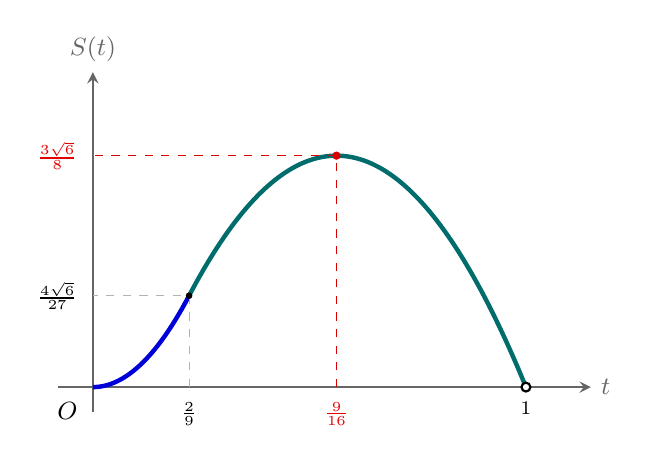
\begin{tikzpicture}[x=5.5cm, y=3.2cm, >=stealth, every node/.style={font=\small}]

    % ============================================================
    % 1. 座標軸
    % ============================================================
    \draw[->, thick, gray!80!black] (-0.08, 0) -- (1.15, 0) node[right] {$t$};
    \draw[->, thick, gray!80!black] (0, -0.1) -- (0, 1.25) node[above] {$S(t)$};
    \node[below left=2pt] at (0, 0) {$O$};

    % ============================================================
    % 2. 曲線 S(t) の描画
    % スケール係数: 最大値 3*sqrt(6)/8 ≈ 0.9185 が y = 0.92 付近になるよう
    % そのままの実数値で描画
    % ============================================================
    % (1) 0 <= t <= 2/9 (放物線: 下に凸 3*sqrt(6)*t^2)
    % 2/9 ≈ 0.2222
    \draw[line width=1.6pt, blue!85!black, domain=0:0.2222, samples=50, smooth]
    plot (\x, {3.0 * sqrt(6) * \x * \x});

    % (2) 2/9 <= t <= 1 (放物線: 上に凸 12*sqrt(6)/49 * (-8t^2 + 9t - 1))
    \draw[line width=1.6pt, teal!85!black, domain=0.2222:1.0, samples=80, smooth]
    plot (\x, {(12.0 * sqrt(6) / 49.0) * (-8.0*\x*\x + 9.0*\x - 1.0)});

    % ============================================================
    % 3. 特徴点・補助線
    % ============================================================
    % 接続点 t = 2/9: S(2/9) = 4*sqrt(6)/27 ≈ 0.363
    \pgfmathsetmacro{\yConn}{4.0 * sqrt(6) / 27.0}
    \draw[dashed, gray!60] (0.2222, 0) -- (0.2222, \yConn) -- (0, \yConn);
    \fill[black] (0.2222, \yConn) circle (1.2pt);
    \node[below=2pt, font=\scriptsize] at (0.2222, 0) {$\frac{2}{9}$};
    \node[left=2pt, font=\scriptsize]  at (0, \yConn) {$\frac{4\sqrt{6}}{27}$};

    % 最大値点 t = 9/16 = 0.5625: S(9/16) = 3*sqrt(6)/8 ≈ 0.9185
    \pgfmathsetmacro{\xMax}{9.0 / 16.0}
    \pgfmathsetmacro{\yMax}{3.0 * sqrt(6) / 8.0}
    \draw[dashed, red!85!black] (\xMax, 0) -- (\xMax, \yMax) -- (0, \yMax);
    \fill[red!85!black] (\xMax, \yMax) circle (1.5pt);

    \node[below=2pt, font=\scriptsize, red!90!black] at (\xMax, 0) {$\frac{9}{16}$};
    \node[left=2pt, font=\scriptsize, red!90!black]  at (0, \yMax) {$\frac{3\sqrt{6}}{8}$};

    % 端点 t = 1: S(1) = 0 (白丸)
    \node[below=2pt, font=\scriptsize] at (1.0, 0) {$1$};
    \fill[white] (1.0, 0) circle (1.6pt);
    \draw[thick, black] (1.0, 0) circle (1.6pt);

  \end{tikzpicture}
  \caption{断面積 $S(t)$ のグラフ}
  \label{fig:cross_section_area_graph}
\end{figure}

\cref{eq:16}より$0 < t \le \dfrac{2}{9}$ の時は$S(t)$は単調増加であり，$t=\dfrac{2}{9}$で連続で，
$\dfrac{2}{9} \le t < 1$ の時は$t = \dfrac{9}{16}$で最大値をとる．従って全体の最大値も$t = \dfrac{9}{16}$の時であり，その最大値は
\begin{align}
  \max S(t) = S\left(\dfrac{9}{16}\right) = \dfrac{3\sqrt{6}}{8}
\end{align}
である．

\end{document}
